\documentclass{beamer}

\usepackage[francais]{babel}
\usepackage[utf8]{inputenc}
\usepackage[T1]{fontenc}
\usepackage{graphicx}
\usepackage{graphics}
\usepackage{color}
\usepackage{textcomp}
\usepackage{pifont}
\usepackage[normalem]{ulem}
\usepackage{times}
\usepackage{hyperref}
\usepackage{verbatim}
\usepackage{amsmath}
\usepackage{amsthm}
\usepackage{amsfonts}
\usepackage[mathscr]{euscript}
\usepackage{pgfpages}
\usepackage{listings}
\usepackage{subfigure}
\usepackage{algorithm}
\usepackage[noend]{algorithmic}
\usepackage{pdftricks}
\usepackage{mathrsfs}
\usepackage{array}
\usepackage{fancybox}
% \usepackage{columns}
\usepackage{multirow}
\usepackage{url}
\usepackage{tikz}
\usepackage{colortbl}
%\usepackage{cite} %DO NOT FUCKING USE CITE ON BEAMER !!! LOST 30 GODDAM' MINUTES ON THIS SHIT !!!
\usepackage{mathabx}
\usepackage{amssymb}
\usepackage{eurosym}
\usepackage{wasysym} % ch0

\let\texteuro\euro

\hypersetup{colorlinks,%
            citecolor=black,%
            filecolor=black,%
            linkcolor=black,%
            urlcolor=blue}

%\addtolength{\parskip}{10pt}

\usetikzlibrary{calc}

\mode<presentation>
\setbeamertemplate{footline}[frame number]
\setbeamercovered{transparent}
\usetheme[navigation]{ESI}

%lst
\definecolor{comment-green}{RGB}{0,166,80}
\lstset{language=C++,
  keywordstyle=\lst@ifdisplaystyle\bf\fi\color{blue!60},
  commentstyle=\color{comment-green},
  stringstyle=\color{red},
  basicstyle=\lst@ifdisplaystyle\tiny\else\tt\fi,
  morekeywords={
    constexpr,concept,decltype,nullptr,nullptr_t,noexcept,final,override},
  frame=single,
  xleftmargin=0.5cm,
  numbers=left,
  tabsize=2}

%title
\subtitle{Langage \texttt{C} / \cpp}
\author{R. Absil}
\date{\today}

%styles
\theoremstyle{definition}
\newtheorem{thm}{Théorème}
\newtheorem{conj}[thm]{Conjecture}
\newtheorem{deff}[thm]{Définition}
\newtheorem{prop}[thm]{Propriété}
\newtheorem{lem}[thm]{Lemme}
\newtheorem*{lem*}{Lemme}
\newtheorem{cor}[thm]{Corollaire}
%\newtheorem{example}{Exemple}
\newtheorem{remark}{Remarque}
\newtheorem{exo}{Exercice}

%typeset
\newcommand{\ie}{{\emph{i.e., }}}
\newcommand{\eg}{{\emph{e.g., }}}
\newcommand{\etal}{{\emph{et al.}}}
\newcommand{\rrceil}{\unichar{"2308}}
\newcommand{\sloand}[2]{\footnote{N. J. A. Sloane - OEIS Foundation - \texttt{www.oeis.org}, Sequence #1 - #2.}}

%math
\newcommand{\IN}{{\mathbb N}}
\newcommand{\IQ}{{\mathbb Q}}
\newcommand{\IR}{{\mathbb R}}
\newcommand{\IZ}{{\mathbb Z}}
\newcommand{\IP}{{\mathbb P}}
\newcommand{\IC}{{\mathbb C}}
\newcommand{\bigo}{{\mathcal{O}}}
\renewcommand{\mod}{\bmod}
\newcommand{\ssi}{\Leftrightarrow}
\newcommand{\then}{\Rightarrow}
\newcommand{\fle}[1]{\stackrel{#1}{\longrightarrow}}
\newcommand{\suchthat}{~\big|~}
\newcommand{\floor}[1]{\left\lfloor #1 \right\rfloor}
\newcommand{\ceil}[1]{\left\lceil #1 \right\rceil}
\DeclareMathOperator*{\argmin}{argmin}
\DeclareMathOperator*{\argmax}{argmax}

%tikz
\tikzstyle{_vertex}=[fill=white, circle,minimum size=12pt,inner sep=1pt]
\tikzstyle{_blackv}=[fill=black, circle,minimum size=8pt,inner sep=1pt]
\tikzstyle{_dot}=[fill=black, circle, minimum size = 1mm, inner sep=0pt]
\tikzstyle{_bigvertex}=[fill=white, circle,minimum size=21pt,inner sep=1pt]
\tikzstyle{_arc}=[->, >=stealth]
\tikzstyle{_boldarc}=[->, >=stealth, line width=2pt]

\newcommand{\cpp}{\texttt{C++}}
\newcommand{\java}{\texttt{Java}}


\title{Ch. 10 - Sémantique de mouvement}

\begin{document}
\begin{frame}
  \titlepage
\end{frame}

\begin{frame}
  \frametitle{Table des matières}
  \footnotesize \tableofcontents[pausesections,pausesubsections]
\end{frame}


\section{Introduction}

\begin{frame}
\frametitle{Le besoin de performances}
\begin{itemize}[<+->]
\item Par défaut, les paramètres sont passés par valeur en \cpp
\end{itemize}
\begin{alertblock}<+->{Problème}
	\begin{itemize}[<+->]
	\item Performances en cas de copie de gros objets
	\end{itemize}
\end{alertblock}
\begin{block}<+->{Solution}
	\begin{itemize}[<+->]
	\item Utiliser le passage par référence
	\item Utiliser le passage par adresse
	\end{itemize}
\end{block}
\begin{itemize}[<+->]
\item Parfois, cette solution ne suffit pas
	\begin{itemize}
	\item Création implicite d'objets temporaires
	\end{itemize}
\end{itemize}
\end{frame}

\begin{frame}
\frametitle{Le problème des temporaires}
\begin{exampleblock}<+->{Exemple de fonction}
	\begin{itemize}
	\item \lstinline|string hello() \{ return string("Hello"); \}|
	\end{itemize}
\end{exampleblock}
\begin{itemize}[<+->]
\item Cette fonction retourne un \texttt{string} par valeur
\item À chaque appel, la fonction
	\begin{enumerate}
	\item Crée un temporaire pour y stocker le littéral \lstinline|"Hello"|
	\item Retourne une copie de ce temporaire
	\end{enumerate}
\item Ça fait beaucoup de temporaires...
\item Ce problème se pose avec toutes les fonctions retournant un gros objet construit localement
\item Solution médiocre : allouer dynamiquement (avec \lstinline|shared_ptr|)
	\begin{itemize}
	\item Plus lent qu'une allocation automatique
	\end{itemize}
\item Excellente solution : utiliser la sémantique de mouvement
	\begin{itemize}
	\item Mis en œuvre par le biais des références de rvalue
	\end{itemize}
\end{itemize}
\end{frame}

\section{Références de rvalue}

\begin{frame}
\frametitle{Le besoin de lvalues}
\begin{itemize}
\onslide<1-> \item Analysons \lstinline|int x = 42;|
	\begin{itemize}
	\onslide<2-> \item $42$ est une rvalue (un littéral)
	\onslide<3-> \item $42$ n'a pas d'adresse
	\onslide<4-> \item On le stocke dans une lvalue pour l'utiliser
	\end{itemize}
\onslide<5-> \item Analysons 
\end{itemize}
\centering\visible<5-|handout:1>{\frame{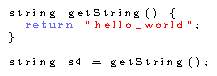
\includegraphics[width=.5\textwidth]{pics/code1.pdf}}}
\begin{itemize}
\onslide<6-> \item Même cas que précédemment
	\begin{itemize}
	\onslide<7-> \item ... mais on utilise un littéral après un appel de fonction
	\onslide<8-> \item On le stocke dans une lvalue pour l'utiliser
	\end{itemize}
\end{itemize}
\end{frame}

\begin{frame}
\frametitle{Le cas des temporaires}
\begin{itemize}
\onslide<1-> \item Analysons \lstinline|int y = x + 1;|
	\begin{itemize}
	\onslide<2-> \item \texttt{x + 1} est une rvalue
	\onslide<3-> \item Le compilateur crée un objet temporaire pour stocker le résultat de l'opérateur \texttt{+}
	\onslide<4-> \item On stocke le temporaire rvalue dans une lvalue
	\end{itemize}
\onslide<5-> \item Analysons
\end{itemize}
\centering\visible<5-|handout:1>{\frame{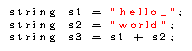
\includegraphics[width=.5\textwidth]{pics/code2.pdf}}}
\begin{itemize}
\onslide<6-> \item Même cas que précédemment
\onslide<7-> \item La gestion des temporaires peut coûter des ressources
	\begin{itemize}
	\onslide<8-> \item Surtout si les temporaires créés sont nombreux / gros
	\end{itemize}
\end{itemize}
\end{frame}

\begin{frame}
\frametitle{Références de \texttt{rvalue}}
\begin{itemize}[<+->]
\item Référence conçue pour être initialisée avec une \texttt{rvalue} seulement
\end{itemize}
\begin{exampleblock}<+->{Syntaxe}
	\begin{itemize}[<+->]
	\item On utilise l'opérateur \texttt{\&\&}
	\item \lstinline|int && x = 5;|
	\item \lstinline|auto && f \{Fraction(2,3)\};|
	\end{itemize}
\end{exampleblock}
\begin{itemize}[<+->]
\item Permet d'étendre la durée de vie d'un temporaire
\item Par le biais de la sémantique de déplacement, elles permettent d'éviter des copies d'objets
\end{itemize}
\end{frame}

\begin{frame}[containsverbatim]
\frametitle{Exemple}
\begin{itemize}
\item Fichier \texttt{rvalue-ref.cpp}
\end{itemize}
\begin{lstlisting}
int main()
{
	string s1 = "Hello ";
	string s2 = "World";
  	
	string && s3 = s1 + s2; //rvalue reference
	cout << s3 << endl;;

	s3 += "!";
	sout << s3 << endl;
}
\end{lstlisting}
\end{frame}

\begin{frame}[containsverbatim]
\frametitle{Règles d'appel}
\begin{itemize}
\item Fichier \texttt{surdef-rvalue-ref.cpp}
\end{itemize}
\begin{lstlisting}
void f(int & lref) // l-value arguments will select this function
{
	cout << "l-value reference" << endl;
}

void f(const int & lref) // const l-value arguments will select this function
{
	cout << "l-value reference to const" << endl;
}
 
void f(int && rref) // r-value arguments will select this function
{
	cout << "r-value reference" << endl;
}
 
int main()
{
	int x{ 5 };
	f(x); // l-value argument calls l-value version of function
	f(5); // r-value argument calls r-value version of function
}
\end{lstlisting}
\end{frame}

\begin{frame}
\frametitle{Création de références}
\begin{itemize}
\onslide<1-> \item On ne peut pas créer de références à partir de n'importe quoi
\onslide<2-> \item Le tableau ci-dessus illustre les créations possibles
\end{itemize}
\onslide<3-> 
\centering
\begin{tabular}{|r|cccc|}
\hline
                      & lvalue & const lvalue & rvalue & const rvalue \\
\hline
\texttt{T\&}          & oui    &              &        &              \\
\texttt{const T\&}    & oui    & oui          & oui    & oui          \\
\texttt{T\&\&}        &        &              & oui    &              \\
\texttt{const T\&\&}  &        &              &        & oui          \\
\hline
\end{tabular}
\begin{itemize}
\onslide<4-> \item En pratique, \lstinline|const T&&| n'est jamais utilisé
	\begin{itemize}
	\onslide<5-> \item Aucun intérêt de « lire depuis un temporaire »
	\end{itemize}
\end{itemize}
\end{frame}

\begin{frame}[containsverbatim]
\frametitle{Forwarding arguments}
\begin{itemize}
\item En \cpp,  étant donné une expression \texttt{E(a1, a2, ... , an)}, il n'est pas possible d'écrire une fonction \texttt{f} telle \linebreak \texttt{f(a1, a2, ... , an)} soit équivalent
	\begin{itemize}
	\item ... pour des raisons techniques
	\end{itemize}
\item On ne peut pas écrire \lstinline|void f1(int && i) {}| et \lstinline|void f2(int&& i) { f1(i); }|
\item Ce problème est appelé le « forwarding problem »
\item Avant les références de \texttt{rvalue}, plusieurs solutions non satisfaisantes existaient
\item Solution : utiliser \texttt{std::forward}
	\begin{itemize}
	\item \lstinline|void f2(int&& i) { f1(std::forward<int>(i)); }|
	\end{itemize}
\item Sucre syntaxique pour \lstinline|static_cast<T&&>(i)|
\item Plus de détails au Ch. 13
\end{itemize}
\end{frame}

\section{Constructeur et affectation de mouvement}

\begin{frame}
\frametitle{Permettre la sémantique de mouvement}
\begin{exampleblock}<+->{Objectif}
	\begin{itemize}[<+->]
	\item On veut éviter au maximum la copie de temporaires
	\end{itemize}
\end{exampleblock}
\begin{itemize}[<+->]
\item On évite cela en utilisant la sémantique de mouvement
	\begin{itemize}
	\item Parfois appelé sémantique de déplacement
	\end{itemize}
\item Mis en œuvre à l'aide de deux outils
	\begin{enumerate}
	\item Constructeur de mouvement
	\item Opérateur d'affectation de mouvement
		\begin{itemize}
		\item Par opposition à opérateur d'affectation de copie
		\end{itemize}
	\end{enumerate}
\item Constructeur et opérateur appelés selon les règles d'appel de fonctions
	\begin{itemize}
	\item Sélectionnés si appelé avec des rvalue
	\end{itemize}
\end{itemize}
\end{frame}

\begin{frame}
\frametitle{Constructeur de mouvement}
\begin{itemize}[<+->]
\item Syntaxe
	\begin{itemize}
	\item \lstinline|T(T&& t)|
	\item \lstinline|T(T&& t) = delete|
	\item \lstinline|T(T&& t) = default|
	\end{itemize}
\item Constructeur de mouvement implicitement généré si toutes les conditions suivantes sont vraies
	\begin{itemize}
	\item Il n'y a ni constructeur de recopie ni opérateur d'affectation de recopie explicite
	\item Il n'y a ni constructeur de mouvement ni opérateur d'affectation de mouvement explicite
	\item Il n'y a pas de destructeur explicite
	\end{itemize}
\item Constructeur de mouvement implicitement \lstinline|= delete| si au moins une des conditions suivantes est vraie
	\begin{itemize}
	\item \texttt{T} a des attributs non statiques qui ne peuvent pas être déplacés
	\item \texttt{T} a une superclasse qui ne peut pas être déplacée ou détruite
	\end{itemize}
\end{itemize}
\end{frame}

\begin{frame}
\frametitle{Opérateur d'affectation de mouvement}
\begin{itemize}[<+->]
\item Syntaxe
	\begin{itemize}
	\item \lstinline|T& operator=(T&& t)|
	\item \lstinline|T& operator=(T&& t) = delete|
	\item \lstinline|T& operator=(T&& t) = default|
	\end{itemize}
\item Opérateur implicitement généré si toutes les conditions suivantes sont vraies
	\begin{itemize}
	\item Il n'y a ni constructeur de recopie ni opérateur d'affectation de recopie explicite
	\item Il n'y a ni constructeur de mouvement ni opérateur d'affectation de mouvement explicite
	\item Il n'y a pas de destructeur explicite
	\end{itemize}
\item Constructeur de mouvement implicitement \lstinline|= delete| si au moins une des conditions suivantes est vraie
	\begin{itemize}
	\item \texttt{T} a des attributs non statiques qui ne peuvent pas être déplacés
	\item \texttt{T} a une superclasse qui ne peut pas être déplacée ou détruite
	\end{itemize}
\end{itemize}
\end{frame}

\begin{frame}[containsverbatim]
\frametitle{Exemple (1/2)}
\begin{itemize}
\item Fichier \texttt{move.cpp}
\end{itemize}
\begin{lstlisting}
struct A
{
    int i;
    
    A(int i = 0) : i(i) { cout << "+" << endl; } //default cstr
    A(const A& a) : i(a.i) { cout << "c" << endl; } //copy cstr
    A(A&& a) : i(std::move(a.i)) {cout << "m" << endl; } //move cstr
    A& operator=(const A& a)
    {
        cout << "=c" << endl;
        if(this != &a)
            i = a.i;
        return *this;
    }
    A& operator=(A&& a)
    {
        cout << "=m" << endl;
        i = std::move(a.i);
        return *this;
    }
};
\end{lstlisting}
\begin{itemize}
\item Désactiver optimisations \texttt{gcc} : \texttt{-fno-elide-constructors}
\end{itemize}
\end{frame}

\begin{frame}[containsverbatim]
\frametitle{Exemple (2/2)}
\begin{itemize}
\item Fichier \texttt{move.cpp}
\end{itemize}
\begin{lstlisting}
//void f(A a) { cout << "by value" << endl; }  //1
void f(A& a) { cout << "by ref" << endl; } //2
void f(const A& a) { cout << "by const ref" << endl; } //2
void f(A&& a) { cout << "by rvalue ref" << endl; } //2

int main()
{
    A a1(1);
    f(a1);
    
    const A a2(2);
    f(a2);
    
    f(A(3));
}
\end{lstlisting}
\begin{itemize}
\item Désactiver optimisations \texttt{gcc} : \texttt{-fno-elide-constructors}
\end{itemize}
\end{frame}

\begin{frame}
\frametitle{Pourquoi tant de haine ?}
\begin{exampleblock}<+->{Question}
	\begin{itemize}[<+->]
	\item Pourquoi implémenter des constructeurs de mouvement si le compilateur optimise ?
	\end{itemize}
\end{exampleblock}
\begin{itemize}[<+->]
\item En pratique, l'une des seules optimisations effectuée est « Return value optimisation »
	\begin{itemize}
	\item Uniquement sur le retour de fonction
	\end{itemize}
\item Pas d'application sur les paramètres de fonctions
\item En particulier, le standard prend régulièrement des références de rvalue en paramètre
\item Si le constructeur de mouvement et l'opérateur d'assignation de mouvement sont implémentés, offre de bonnes optimisations
\item \texttt{std::move} permet de « déplacer » une rvalue
	\begin{itemize}
	\item En pratique, convertit une lvalue en rvalue
	\item Ne crée pas de temporaire
	\end{itemize}
\end{itemize}
\end{frame}

\begin{frame}[containsverbatim]
\frametitle{Erreur courante}
\begin{itemize}
\item Ne faites pas ça
\end{itemize}
\begin{lstlisting}
A create_A()
{
	A a;
	return std::move(a);
}
\end{lstlisting}
\begin{itemize}
\item Et \emph{surtout pas} ça
\end{itemize}
\begin{lstlisting}
A&& create_A()
{
	A a;
	return std::move(a);
}
\end{lstlisting}
\begin{itemize}
\item Les déplacements sont exclusivement effectués par le constructeur de déplacement (implicitement)
\end{itemize}
\end{frame}

\section{La sémantique de mouvement}

\begin{frame}
\frametitle{Hygiène}
\begin{itemize}[<+->]
\item En pratique, dès qu'une classe « gère une ressource », elle \emph{doit} au moins implémenter 
	\begin{enumerate}
	\item un destructeur
	\item un constructeur de recopie
	\item un opérateur d'affectation de copie
	\end{enumerate}
\item Si l'on a besoin de l'un, on a besoin des trois
\item Pour des raisons d'optimisation, on veut parfois
	\begin{enumerate}
	\item un constructeur de mouvement
	\item un opérateur d'affectation de mouvement
	\end{enumerate}
\item Ressource : wrapper, mémoire dynamique, pointeur, mutex, etc.
\item Critères de qualité
	\begin{itemize}
	\item Éviter la duplication de code
	\item Garantie forte d'exception
	\end{itemize}
\end{itemize}
\end{frame}

\begin{frame}
\frametitle{Rules of three / five / zero}
\begin{exampleblock}<+->{La règle des trois}
	\begin{itemize}[<+->]
	\item Si une classe a besoin d'un destructeur, d'un constructeur de recopie ou d'un opérateur d'affectation de copie, elle a besoin des trois	
	\end{itemize}
\end{exampleblock}
\begin{exampleblock}<+->{La règle des cinq}
	\begin{itemize}[<+->]
	\item Si une classe a besoin d'un constructeur de mouvement ou d'un opérateur d'affectation de mouvement, elle a besoin
		\begin{itemize}
		\item de la règle des trois
		\item d'un constructeur de mouvement \emph{et} d'un opérateur d'affectation de mouvement
		\end{itemize}
	\end{itemize}
\end{exampleblock}
\begin{itemize}[<+->]
\item L'idiôme « copy and swap » permet de fournir des critères de qualité
\end{itemize}
\end{frame}

\begin{frame}
\frametitle{Dans la plupart des cas}
\begin{itemize}[<+->]
\item Dans la plupart des cas, les classes ne « gèrent pas de ressources »
	\begin{itemize}
	\item Pas de wrappers, de pointeurs (intelligents ou non), de mutex, etc.
	\end{itemize}
\item Dans ce cas, il n'est pas nécessaire d'implémenter
	\begin{itemize}
	\item la règle des trois
	\item la règle des cinq
	\end{itemize}
\item Les sémantiques de copie et de déplacement sont implémentées correctement par défaut
\item Si une classe ne bénéficie pas de la sémantique de mouvement, il n'est pas non plus nécessaire de l'implémenter
%	\begin{itemize}
%	\item Classes peu volumineuses
%	\end{itemize}
\item Le principe POO de responsabilité unique implique également qu'une classe gérant une ressource doivent \emph{uniquement} s'occuper de cette gestion
	\begin{itemize}
	\item « Règle de zéro » pour les autres classes
	\end{itemize}
\end{itemize}
\end{frame}

\begin{frame}
\frametitle{Construction d'un exemple académique}
\begin{itemize}
\item On veut créer une classe modélisant un tableau à taille statique d'entiers
	\begin{itemize}
	\item Sans utiliser les conteneurs, qui implémentent la règle des cinq
	\end{itemize}
\item Fonctionnalités :
	\begin{itemize}
	\item un constructeur, qui alloue la mémoire dynamiquement
	\item un opérateur \texttt{[]}, qui permet l'accès et l'affectation	
	\end{itemize}
\item Cette classe est de taille « arbitrairement grande »
	\begin{itemize}
	\item On parle ici de l'espace total alloué, pas du résultat de \lstinline|sizeof|
	\end{itemize}
\end{itemize}
\end{frame}

\begin{frame}[containsverbatim]
\frametitle{La base}
\begin{itemize}
\item Fichier \texttt{static-array.cpp}
\end{itemize}
\begin{lstlisting}
class Array
{
    unsigned _size;
    int * data;
    
    public:
        Array(unsigned size = 0)
            : _size(size),
              data(size != 0 ? new int[size] : nullptr)
        {}
    
        int& operator[](unsigned pos) 
        { 
        	return data[pos]; 
        }        
        
        int size() const 
        { 
        	return _size; 
        }
        
    ...
};
\end{lstlisting}
\end{frame}

\begin{frame}
\frametitle{Debriefing d'analyse}
\begin{exampleblock}<+->{Constatations}
\begin{itemize}[<+->]
\item On veut sûrement passer le plus souvent possible \texttt{Array} par référence
	\begin{itemize}
	\item Classe assez volumineuse
	\item Si on compte les données allouées avec \lstinline|new|
	\end{itemize}
\item Il faut implémenter la règle des trois si l'on veut
	\begin{itemize}
	\item que la copie et l'affectation recopie soient fonctionnelles
	\item éviter les fuites mémoires
	\end{itemize}
\item Il faut implémenter la règle des cinq si l'on veut éviter des copies de temporaires inutiles
\end{itemize}
\end{exampleblock}
\begin{itemize}[<+->]
\item Pour des raisons académiques, on implémentera une fonction \texttt{create\_increasing\_array(n)}, qui crée un tableau d'éléments [0, ..., n-1]
\end{itemize}
\end{frame}

\begin{frame}[containsverbatim]
\frametitle{La règle des trois}
\begin{itemize}
\item Fichier \texttt{static-array.cpp}
\end{itemize}
\begin{lstlisting}
~Array()
{
     if(data)
         delete[] data;
}
    
Array& operator=(const Array& a)
{
     if(this != &a)
     {
          if(data)
               delete[] data;
                
          _size = a._size;
          data = a._size != 0 ? new int[a._size] : nullptr;
          std::copy(a.data, a.data + _size, data);
     }
           
     return *this;
}
    
Array(const Array& a) : _size(a._size), data(a._size != 0 ? new int[a._size] : nullptr)
{
     std::copy(a.data, a.data + _size, data);
}
\end{lstlisting}
\end{frame}

\begin{frame}[containsverbatim]
\frametitle{La règle des cinq}\begin{itemize}
\item Fichier \texttt{static-array.cpp}
\end{itemize}
\begin{lstlisting}
Array(Array && a) :
     _size(std::move(a._size)),
     _data(std::move(a._data))
{            
     a._data = nullptr; //ask why I should do this
}
    
Array& operator=(Array && a)
{
     _size = std::move(a._size);
     _data = std::move(a._data);
     a._data = nullptr;            
            
     return *this;
}
\end{lstlisting}
\begin{itemize}
\item Bonne pratique : utiliser \texttt{std::move} dans l'implémentation de la sémantique de déplacement
\end{itemize}
\end{frame}

\begin{frame}
\frametitle{Debriefing de conception}
\begin{alertblock}<+->{Problème}
\begin{itemize}[<+->]
\item Cela fait \emph{vraiment} beaucoup de copier / coller
\end{itemize}
\end{alertblock}
\begin{itemize}[<+->]
\item Il faut trouver une solution
\end{itemize}
\end{frame}

\section{Idiomes}

\begin{frame}
\frametitle{\cpp\ et les idiomes}
\begin{itemize}[<+->]
\item \cpp\ est un langage qui requiert une bonne hygiène de programmation
\item Une bonne partie de cette hygiène est implémentée via des «~idiomes~»
\item Idiome : forme de conception d'un fragment de code afin d'y intégrer des critères de qualité
\end{itemize}
\begin{exampleblock}<+->{Objectif courant}
	\begin{itemize}[<+->]
	\item Implémenter la règle des cinq et éviter le copier / coller
	\end{itemize}
\end{exampleblock}
\begin{itemize}[<+->]
\item On requiert souvent les constructeurs de déplacement à être \lstinline|noexcept|
	\begin{itemize}
	\item Le standard choisit souvent le constructeur de recopie si le constructeur de déplacement n'est pas \lstinline|noexcept|
	\end{itemize}
\end{itemize}
\end{frame}

\subsection{Copy and swap}

\begin{frame}
\frametitle{La clé}
\begin{itemize}[<+->]
\item Si on a besoin d'implémenter la règle des cinq, l'astuce réside dans
	\begin{enumerate}
	\item l'implémentation d'une fonction \texttt{swap} (souvent amie)
	\item le passage par valeur du paramètre de l'opérateur d'affectation de recopie
	\end{enumerate}
\end{itemize}
\begin{block}<+->{Hygiène \cpp}
	\begin{itemize}[<+->]
	\item Si une copie doit être faite, faites-la grâce au passage par valeur plutôt que manuellement
	\item Offre des optimisations compilatoires
	\end{itemize}
\end{block}
\begin{itemize}[<+->]
\item Hormis l'implémentation de la règle des cinq, le reste de la classe ne change pas
\end{itemize}
\end{frame}

\begin{frame}[containsverbatim]
\frametitle{Illustration}
\begin{itemize}
\item Fichier \texttt{static-array-copy-and-swap.cpp}
\end{itemize}
\begin{lstlisting}
~Array()
{
	if(data)
		delete[] data;
}
    
friend void swap(Array& a1, Array& a2) noexcept
{
	std::swap(a1.size, a2.size);   
	std::swap(a1.data, a2.data);   
}
\end{lstlisting}
\begin{itemize}
\item Bonne pratiques
	\begin{enumerate}
	\item Utiliser \texttt{std::swap} dans l'implémentation d'une fonction \texttt{swap}
	\item Rendre \texttt{swap} \lstinline|noexcept| pour l'utiliser dans le constructeur de déplacement
	\end{enumerate}
\end{itemize}
\end{frame}

\begin{frame}[containsverbatim]
\frametitle{Illustration}
\begin{itemize}
\item Fichier \texttt{static-array-copy-and-swap.cpp}
\end{itemize}
\begin{lstlisting}
Array& operator=(Array a)
{
	swap(*this, a);
            
	return *this;
}
    
Array(const Array& a) : size(a.size), data(a.size != 0 ? new int[a.size] : nullptr)
{
	std::copy(a.data, a.data + size, data);
}
    
Array(Array && a) noexcept
{
	swap(*this, s);
	a.data = nullptr;
}
\end{lstlisting}
\end{frame}

\begin{frame}
\frametitle{Débriefing}
\begin{enumerate}[<+->]
\item Le destructeur n'a pas changé
\item Le constructeur de recopie n'a pas changé
\item On a une fonction \texttt{swap}
\item L'opérateur d'affectation prend son paramètre par valeur
	\begin{itemize}
	\item Effectue une copie
	\item On utilise \texttt{swap} pour échanger \lstinline|*this| et la copie
	\end{itemize}
\item Le constructeur de mouvement utilise \texttt{swap} pour échanger \lstinline|*this| et son paramètre
	\begin{itemize}
	\item Effet de bord (mais c'est correct)
	\item Ne pas oublier (dans ce cas) de mettre 
	\end{itemize}
\item Pas de besoin nécessaire d'opérateur d'affectation de mouvement
	\begin{itemize}
	\item On aurait pu en écrire un
	\item En l'état, utilise le constructeur de déplacement
	\end{itemize}
\end{enumerate}
\end{frame}

\subsection{RAII}

\begin{frame}
\frametitle{L'objectif}
\begin{itemize}[<+->]
\item Parfois, un extrait de code a besoin d'acquérir une ressource
	\begin{itemize}
	\item Un descripteur de fichier
	\item Un sémaphore (mutex)
	\end{itemize}
\item Il est primordial que la ressource 
	\begin{enumerate}
	\item soit bien acquise pour le code qui en a besoin
	\item soit bien libérée quand on a fini le traitement
	\end{enumerate}
\item Ce qui peut mal se passer
	\begin{itemize}
	\item Erreur d'entrée sortie
	\item Impossibilité d'allocation mémoire
	\item Exception non rattrapée
	\end{itemize}
\end{itemize}
\end{frame}

\begin{frame}
\frametitle{L'idiome RAII}
\begin{exampleblock}<+->{Ressource acquisition is initialisation}
	\begin{itemize}[<+->]
	\item Encapsuler une ressource au sein d'une classe	
	\item Utilisation cette ressource via une instance de la classe
	\item Libération de la ressource quand l'objet est détruit
	\end{itemize}
\end{exampleblock}
\begin{itemize}[<+->]
\item La ressource est souvent initialisée et acquise dans le constructeur
	\begin{itemize}
	\item La ressource peut être également allouée ailleurs et passée en paramètre
	\end{itemize}
\item L'objet gérant la source est automatique
	\begin{itemize}
	\item Car ce sont les seuls objets à durée de vie clairement définie au sein d'un bloc
	\end{itemize}
\item Quand l'objet est hors de portée (sortie de bloc), la ressource est libérée
	\begin{itemize}
	\item Via le destructeur
	\end{itemize}
\end{itemize}
\end{frame}

\begin{frame}[containsverbatim]
\frametitle{Exemple académique 1}
\begin{itemize}
\item On suppose que \texttt{m} est un mutex
\end{itemize}
\begin{lstlisting} 
void wrong()
{
    m.lock();                    
    f();                    //wrong 1                  
    if(!everything_ok())    
    	return;             //wrong 2
    m.unlock();                  
}
\end{lstlisting}
\begin{lstlisting}
void right()
{
    std::lock_guard<std::mutex> lk(m); // RAII class
    f();                               // ok
    if(!everything_ok()) 
    	return;                        // ok
}
\end{lstlisting}
\begin{itemize}
\item Source : Cppreference.com
\end{itemize}
\end{frame}

\begin{frame}
\frametitle{Exemple académique 2}
\begin{itemize}[<+->]
\item On veut implémenter une classe permettant de lire des caractères dans un fichier texte
	\begin{itemize}
	\item Académique : sans utiliser \texttt{std::ifstream}
	\end{itemize}
\item Ressources à gérer
	\begin{itemize}
	\item Le descripteur de fichier
	\item Le buffer de lecture
	\end{itemize}
\item On va lire avec \texttt{cstdio.h}
	\begin{itemize}
	\item \texttt{FILE*} : pointeur vers un descripteur de fichier
	\item \texttt{fopen} et \texttt{fclose} : ouvre et ferme le fichier
		\begin{itemize}
		\item Obtient le descripteur, ou le libère
		\end{itemize}
	\item \texttt{fread} : lit des bytes en entrée et les place dans un buffer
	\end{itemize}
\item On veut pouvoir déplacer une instance, mais pas la copier
	\begin{itemize}
	\item Courant comme pratique RAII
	\item Limite les problèmes de synchronisation
	\end{itemize}
\end{itemize}
\end{frame}

\begin{frame}[containsverbatim]
\frametitle{Exemple académique 2}
\begin{itemize}
\item Fichier \texttt{raii.cpp}
\end{itemize}
\begin{lstlisting}
class FileReader {
    std::FILE* f; //old school (C-style) file management
    char * buffer;      
    public:
        FileReader(const char* name) : f(fopen(name, "r+")), buffer(new char[16]) {
            ...
        }
    
        ~FileReader() {
            std::fclose(f); //flush  and free file descriptor
            if(buffer) {
                delete[] buffer;                
                buffer = nullptr;
            }
        }
    
        FileReader(const FileReader& fh) = delete;    
        FileReader& operator=(const FileReader&) = delete;
        
        FileReader(FileReader&& fh) noexcept :
            f(std::move(fh.f)),
            buffer(std::move(fh.buffer)) 
        {
            fh.buffer = nullptr;
        }
};
\end{lstlisting}
\end{frame}
\end{document}
